
\newpage
\chapter{چگونگی پردازش تصاویر در نواحی اولیه قشر بینایی}
    \section{مقدمه}
        یکی از جنبه های مهم علوم اعصاب محاسباتی شامل مدل سازی نحوه تفسیر و پردازش محرک های بصری توسط سیستم بینایی است. مراحل اولیه پردازش بصری در شبکیه و قشر بینایی اولیه 
        (V1) 
        رخ می دهد، جایی که اطلاعات بصری پیچیده ابتدا به الگوهای معنی دار کدگشایی می شوند. این پروژه بر شبیه سازی مکانیسم های پردازش تصویر لایه اول مسیر بصری با استفاده از فیلترهای تفاوت گاوسی 
        (DoG)\footnote{\lr{Difference of Gaussian}}
        و فیلترهای گبور
        \footnote{Gabor}
        تمرکز دارد.

        شبکیه و مسیر بینایی اولیه به طور گسترده مورد مطالعه قرار گرفته اند تا بفهمند که چگونه ورودی های بصری خام به نمایش های ساختاری تبدیل می شوند. در این مرحله، نورون ها میدان های دریافتی را نشان می دهند که به طور انتخابی به ویژگی های بصری مختلف مانند لبه ها، جهت گیری ها و فرکانس های فضایی پاسخ می دهند. دو مدل برجسته که این ویژگی‌ها را نشان می‌دهند، فیلتر تفاضل گاوسی 
        (DoG) 
        و فیلترهای گبور هستند.
        
        فیلترهای 
        DoG 
        برای مدل‌سازی میدان‌های گیرنده در اطراف سلول‌های گانگلیونی شبکیه و نورون‌های هسته ژنیکوله جانبی 
        (LGN) 
        استفاده می‌شوند. این فیلترها با برجسته کردن مناطقی که شدت تغییر سریع دارند، کنتراست را برجسته می‌کنند و به طور موثر لبه‌ها و کنتراست‌های محلی را در صحنه بصری تشخیص می‌دهند. فیلترهای 
        DoG 
        با تقلید از سازمان محیطی مرکز، راه بیولوژیکی قابل قبولی را برای پیش پردازش اطلاعات بصری، کاهش افزونگی و افزایش ویژگی های برجسته ارائه می دهند.
        
        از سوی دیگر، فیلترهای گبور در مدل‌سازی میدان‌های گیرنده انتخابی جهت‌گیری موجود در قشر بینایی اولیه 
        (V1) 
        ابزاری هستند. این فیلترها می‌توانند جهت‌گیری‌ها و فرکانس‌های فضایی خاص را در ورودی بصری شناسایی کنند، که دقیقاً با ویژگی‌های تنظیم سلول‌های ساده در 
        V1 
        مطابقت دارد. بنابراین، فیلترهای گبور می‌توانند ماهیت چگونگی پردازش لبه‌ها و بافت‌ها توسط قشر بینایی را به تصویر بکشند و در مراحل اولیه ادراک بصری و تشخیص الگوی نقش داشته باشند.
        
        در این پروژه، فیلترهای 
        DoG و Gabor 
        را برای شبیه سازی مراحل اولیه پردازش بصری پیاده سازی کردیم. پیاده سازی شامل ایجاد این فیلترها، اعمال آنها بر روی تصاویر ورودی مختلف و تجزیه و تحلیل خروجی های آنها برای درک نقش آنها در پردازش بصری است.
        
        با بررسی قابلیت‌های فیلترهای 
        DoG و Gabor، 
        این مطالعه با هدف پر کردن شکاف بین بینایی بیولوژیکی و مدل‌های محاسباتی، ارائه درک جامعی از فرآیندهای اساسی زیربنای ادراک بصری است. در بخش‌های بعدی روش‌شناسی، پیاده‌سازی و نتایج به‌کارگیری این فیلترها برای محرک‌های بصری را به تفصیل شرح داده می‌شود.
    \section{فیلتر تفاضل گاوسی}
    اولین لایه مسیر بینایی که به شبکیه معروف است، نقش مهمی در مراحل اولیه پردازش تصویر دارد. این لایه وظیفه جذب نور و تبدیل آن به سیگنال های عصبی را بر عهده دارد که سپس برای تفسیر بیشتر به مغز منتقل می شود. یکی از جنبه های کلیدی این پردازش شامل تمایز اطلاعات بصری، به ویژه تشخیص لبه ها و تضادها در میدان بینایی است. یکی از مدل‌های محاسباتی مؤثر که این فرآیند بیولوژیکی را تقلید می‌کند، فیلتر تفاوت گاوسی 
    (DoG) 
    است.

    فیلتر 
    DoG 
    از میدان‌های گیرنده سلول‌های گانگلیونی شبکیه الهام گرفته شده است که برای تشخیص لبه و افزایش کنتراست در سیستم بینایی ضروری است. سلول های گانگلیونی در شبکیه، نورون های تخصصی هستند که اطلاعات بصری را قبل از ارسال به مغز پردازش می کنند. این سلول‌ها دارای میدان‌های گیرنده هستند که شامل یک ناحیه مرکزی است که توسط نور برانگیخته یا مهار می‌شود و یک ناحیه اطراف آن که واکنش مخالف را نشان می‌دهد. این مکانیسم به سلول‌های گانگلیونی اجازه می‌دهد لبه‌ها و تغییرات شدت نور را تشخیص دهند و نقش مهمی در ادراک بصری ایفا کنند.

    فیلتر 
    DoG 
    به طور ریاضی مکانیسم سلول‌های گانگلیونی را با کم کردن یک تاری گاوسی وسیع‌تر 
    (نماینده اطراف) 
    از یک تاری گاوسی باریکتر 
    (نماینده مرکز) 
    شبیه‌سازی می‌کند. این تفریق لبه‌ها و جزئیات ظریف ورودی بصری را افزایش می‌دهد، شبیه به پردازش انجام شده توسط سلول‌های گانگلیونی شبکیه. با تقلید از رفتار این سلول ها، فیلترهای 
    DoG 
    روشی قوی برای برجسته کردن مناطق با کنتراست بالا و سرکوب مناطق یکنواخت در یک تصویر ارائه می کنند.
    (شکل \ref{fig:part1-ganglion-cells-schematic})
    \begin{figure}[!ht]
        \centering
        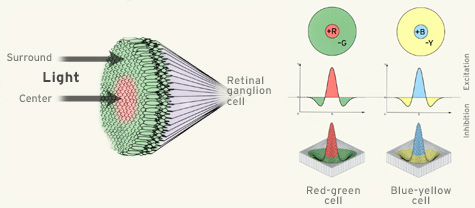
\includegraphics[width=0.8\textwidth]{images/ganglion-cells.jpg} 
        \captionsetup{width=.8\linewidth}
        \caption{\textbf{شمای کلی از سلول های گانگلیونی و ارتباط آن ها با فیلتر 
        DoG.}}
        \label{fig:part1-ganglion-cells-schematic}
    \end{figure}
    در این بخش پروژه، فیلترهای 
    DoG 
    را برای مدل‌سازی پردازش تصویری که در لایه اول مسیر بصری رخ می‌دهد، پیاده‌سازی کردیم. هدف اجرای ما تکرار عملکرد بیولوژیکی سلول‌های گانگلیونی شبکیه است و بینش‌هایی در مورد اینکه چگونه سیستم بینایی انسان به طور موثر اطلاعات بصری را شناسایی و پردازش می‌کند، ارائه می‌کند. از طریق این رویکرد محاسباتی، ما اثربخشی فیلترهای 
    DoG 
    را در بهبود ویژگی‌های تصویر بررسی می‌کنیم و زمینه را برای تحقیقات بیشتر در مورد مکانیسم‌های پردازش بصری پیچیده‌تر فراهم می‌کنیم.

    \subsection{دیدگاه ریاضی}
        در علم تصویربرداری، تفاوت گاوسی ها 
        (DoG) 
        یک الگوریتم بهبود ویژگی است که شامل تفریق یک نسخه تار گاوسی یک تصویر اصلی از نسخه دیگر، کمتر تار شده اصلی است. در مورد ساده تصاویر مقیاس خاکستری، تصاویر تار با انحراف تصاویر اصلی در مقیاس خاکستری با هسته
        \footnote{kernel}
        های گاوسی با عرض متفاوت 
        (انحرافات استاندارد) 
        به دست می آیند. محو کردن یک تصویر با استفاده از هسته گاوسی فقط اطلاعات مکانی با فرکانس بالا را سرکوب می کند. با کم کردن یک تصویر از تصویر دیگر، اطلاعات فضایی که بین محدوده فرکانس‌هایی که در دو تصویر تار حفظ می‌شوند، حفظ می‌شود. بنابراین، 
        DoG 
        یک فیلتر  میان‌گذر فضایی است که فرکانس‌های تصویر اصلی مقیاس خاکستری را که دور از مرکز هستند، کاهش می‌دهد.
 
        $\Phi_t : \mathbb{R}^n \rightarrow \mathbb{R}$ 
        را به عنوان تابع گاوسی شعاعی 
        $\Phi_t(x) = \mathcal{N}(x|0, t)$ 
        با میانگین 
        $0$ 
        و واریانس 
        $t$، 
        یعنی، تابع گاوسی چندمتغیره 
        $\Phi_t(x) = \mathcal{N}(x|0, tI)$ 
        با میانگین 
        $0$ 
        و کوواریانس 
        $tI$ 
        در نظر بگیرید. به طور صریح‌تر، داریم
        \[
        \Phi_t(x) = \frac{1}{(2\pi t)^{n/2}} e^{-\frac{|x|^2}{2t}}.
        \]
        تفاوت گاوسی‌ها با واریانس‌های 
        $t_1 < t_2$ 
        تابع هسته
        \[
        K_{t_1, t_2} = \Phi_{t_1} - \Phi_{t_2}
        \]
        است که با تفریق گاوسی با واریانس بالاتر از گاوسی با واریانس کمتر به دست می‌آید. تفاوت عملگر گاوسی همان عملگر کانولوشن مرتبط با این تابع هسته‌ای است. شکل کلی این فیلتر در شکل 
        \ref{fig:part1-DoG}
        نشان داده شده است.
        \begin{figure}[!ht]
            \centering
            \begin{subfigure}[b]{0.4\textwidth}
                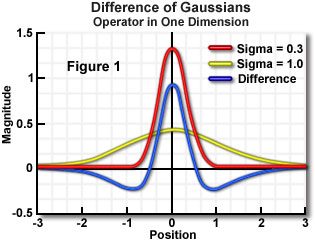
\includegraphics[width=\textwidth]{images/DoG-filter.jpg}
                \caption{شکل کلی نحوه انجام تفاضل گاوسی}
                \label{fig:part1-DoG-filter}
            \end{subfigure}
            \hfill % optional; use for aligning images side by side
            \begin{subfigure}[b]{0.4\textwidth}
                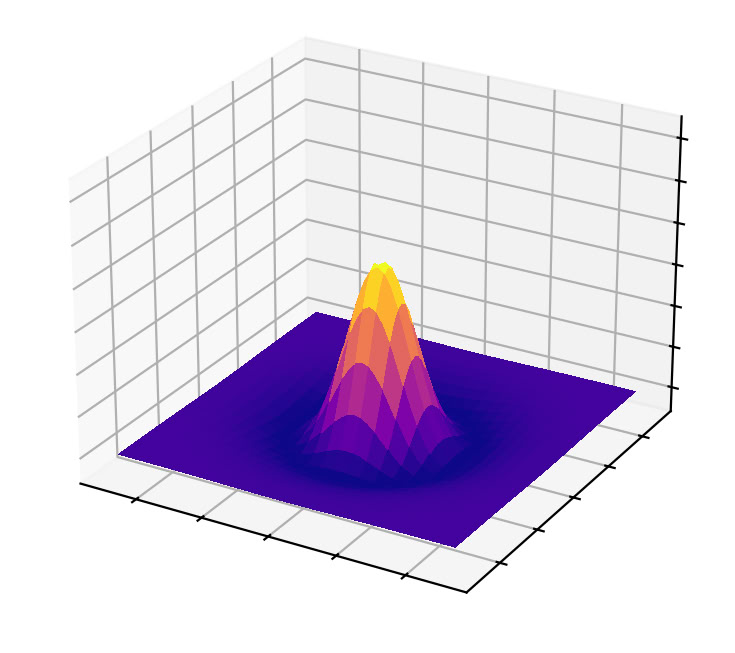
\includegraphics[width=\textwidth]{images/DoG-3d.jpg}
                \caption{شکل ۳ بعدی تفاضل گاوسی}
                \label{fig:part1-DoG-3d}
            \end{subfigure}
            \caption{ تفاضل گاوسی (DoG)}
            \label{fig:part1-DoG}
        \end{figure}
        \subsection{تاثیر پارامتر ها}
            حال در این قسمت تاثیر هر یک از پارامتر ها در فیلتر ها را بررسی می‌کنیم. ما بر نقش دو پارامتر کلیدی تمرکز می کنیم: انحرافات استاندارد دو فیلتر گاوسی اعمال شده. تأثیر آن‌ها بر نتیجه فرآیند فیلتر کردن 
            DoG 
            از طریق مجموعه‌ای از آزمایش‌های طراحی‌شده به‌صورت روش‌مند تحلیل می‌شود و نشان می‌دهد که چگونه تغییرات در این پارامترها بر حساسیت و ویژگی تشخیص لبه تأثیر می‌گذارد.(شکل \ref{fig:part1-DoG-Kernel})

            \begin{figure}[!ht]
                \centering
                \includegraphics[width=\textwidth]{plots/part1-DoG-Kernel.pdf} 
                \captionsetup{width=.9\linewidth}
                \caption{\textbf{مقایسه تاثیر پارامتر های فیلتر DoG.} 
                این شکل سه فیلتر 
                DoG 
                را با مقادیر سیگما متفاوت نشان می‌دهد تا تأثیر آنها بر قابلیت‌های تشخیص لبه را نشان دهد. شکل بالایی یک هسته با $\sigma_1=3 $و $\sigma_2=6 $
                را نشان می دهد که برای تشخیص جزئیات بسیار ایده آل است. شکل میانی با 
                $\sigma_1=4 $و $\sigma_2=8$ 
                پاسخ وسیع تری را برای لبه های برجسته نشان می دهد. شکل پایین دارای یک هسته خارج از مرکز با 
                $\sigma_1=6$ و $\sigma_2=3$ 
                است که حساسیت به ویژگی های جهت را افزایش می دهد. هر فیلتر به صورت سه بعدی نیز برای درک بهتر آمده است.}
                \label{fig:part1-DoG-Kernel}
            \end{figure}
        \subsection{خروجی تصویر پس از اعمال فیلتر DoG}
            حال در این بخش، یک فیلتر 
            DoG 
            را روی یک تصویر نمونه اعمال کرده و خروجی آن را نشان می‌دهیم. برای اینکار، یک تصویر نمونه که از مخزن دانشگاه واترلو 
            \footnote{\href{https://links.uwaterloo.ca/Repository.html}{https://links.uwaterloo.ca/Repository.html}}
            انتخاب کرده و فیلتر 
            DoG 
            را با اندازه های مختلف و همچنین دو نسخه 
            on-center 
            و 
            off-center 
            را روی آن هم‌گشت
            \footnote{Convolution}
            می‌کنیم. 

            شکل
            \ref{fig:part1-DoG-on-image}
            کاربرد فیلتر تفاوت گوسی ها 
            (DoG) 
            را بر روی یک تصویر نمونه نشان می دهد، که اثرات آن را با مقادیر مختلف سیگما و کنتراست نسخه های 
            on-center
            و 
            off-center
            نشان می دهد.

            تصویر ورودی که در بالا سمت چپ نشان داده شده است، به عنوان محرک بصری اصلی برای فرآیندهای فیلتر بعدی عمل می کند. در مجاورت این تصویر، هسته 
            DoG 
            نشان داده شده است که با تفریق دو تابع گاوسی با انحرافات استاندارد مختلف 
            (سیگما) 
            ساخته شده است. این هسته برای شبیه سازی خواص میدان پذیرای سلول های گانگلیونی شبکیه است.

            در ردیف وسط، خروجی فیلتر 
            DoG 
            با نسخه
            on-center
            ارائه شده است. این نسخه بر نواحی تأکید دارد که بخش مرکزی میدان گیرنده توسط نور برانگیخته می شود و به طور مؤثر لبه ها و جزئیات ظریف درون تصویر را برجسته می کند. مقادیر مختلف سیگما برای نشان دادن اینکه چگونه گستردگی توابع گاوسی بر تشخیص لبه‌ها تأثیر می‌گذارد نیز در ردیف پایین اعمال می‌شود، با سیگماهای کوچکتر که جزئیات ریزتر را افزایش می‌دهند و سیگماهای بزرگ‌تر ساختارهای وسیع‌تری را جذب می‌کنند.

            ستون اول از سمت راست خروجی 
            off-center
            فیلتر 
            DoG 
            را نشان می دهد. در اینجا، فیلتر تنظیم شده است تا مناطقی را که بخش مرکزی میدان گیرنده توسط نور مهار می شود، بهبود بخشد، و در نتیجه تضاد تکمیلی با خروجی در مرکز ایجاد می کند. تغییر در مقادیر سیگما به طور مشابه بر سطح جزئیات و میزان تشخیص لبه تأثیر می‌گذارد و انعطاف‌پذیری فیلتر 
            DoG 
            را در مدل‌سازی جنبه‌های مختلف پردازش بصری نشان می‌دهد.

            \begin{figure}[!ht]
                \centering
                \includegraphics[width=0.95\textwidth]{plots/part1-DoG-convolution.pdf} 
                \captionsetup{width=.9\linewidth}
                \caption{\textbf{کاربرد تفاضل فیلتر گاوسی 
                (DoG) 
                روی یک تصویر نمونه.} 
                شکل، فرآیند و اثرات اعمال فیلتر 
                DoG 
                بر روی یک تصویر ورودی را نشان می دهد. 
                (ستون اول از سمت چپ) 
                تصویر ورودی اصلی که برای فیلتر کردن استفاده می شود. 
                (ستون دوم از سمت چپ) 
                هسته 
                DoG 
                با تفریق دو تابع گاوسی با انحرافات استاندارد مختلف (سیگما) 
                ایجاد شده است. 
                (ستون سوم از سمت چپ) 
                خروجی فیلتر 
                DoG 
                نسخه 
                on-center، 
                برجسته کردن لبه ها و جزئیات دقیق. مقادیر مختلف سیگما تأثیر بر تشخیص لبه و افزایش جزئیات را نشان می دهد. 
                (ستون جهارم از سمت چپ) 
                خروجی فیلتر 
                DoG 
                با نسخه
                off-center
                ، با تاکید بر مناطقی که مرکز توسط نور مهار می شود، و تضاد مکملی را با خروجی در مرکز نشان می دهد. تغییرات در مقادیر سیگما نشان داده شده است که انعطاف‌پذیری فیلتر 
                DoG 
                را در مدل‌سازی جنبه‌های مختلف پردازش بصری منعکس می‌کند.
                همانطور که مشاهده می‌کنیم، هر چه مقدار سیگما کوچکتر باشد، لبه های استخراج شده از تصویر نیز نازک تر است. با بزرگتر شدن این مقادیر در ستون دوم، تصویر حاصل نیز دارای خطوطی با ضخامت بیشتر می‌شود. }
                \label{fig:part1-DoG-on-image}
            \end{figure}

    \clearpage
    \section{فیلتر گبور}
        فیلترهای گبور ابزارهای محاسباتی هستند که به طور گسترده به دلیل توانایی آنها در شبیه سازی خواص میدان پذیری نورون ها در قشر بینایی اولیه 
        (V1) 
        شناخته شده است. این فیلترها که به نام دنیس گبور، که آنها را در سال 1946 معرفی کرد، نامگذاری شده‌اند، از آن زمان به بعد در درک چگونگی تفسیر اطلاعات بصری توسط مغز یکپارچه شده‌اند.

        فیلترهای گبور با توانایی آنها در گرفتن مکان یابی فضایی، انتخاب جهت گیری و تنظیم فرکانس فضایی مشخص می شوند، ویژگی هایی که بسیار با الگوهای پاسخ سلول های ساده در 
        V1 
        سازگار است. هر فیلتر گبور در اصل یک موج صفحه سینوسی است که توسط یک پوشش گاوسی ماژوله شده است.
        (گویی فیلتر 
        DoG 
        در یکی از محور های افقی خود کشیده شده است.
        شکل \ref{fig:part1-Gabor})
        این ترکیب به فیلتر اجازه می‌دهد تا به فرکانس‌ها و جهت‌گیری‌های فضایی خاص پاسخ دهد و آن را به ابزاری مؤثر برای تشخیص لبه، تحلیل بافت و استخراج ویژگی در تصاویر تبدیل می‌کند.
        
        از نظر ریاضی، یک فیلتر گبور را می توان به عنوان یک تابع نمایی پیچیده ضرب در یک تابع گاوس توصیف کرد. مولفه سینوسی لبه ها و خطوط را در یک جهت و مقیاس خاص تشخیص می دهد، در حالی که مولفه گاوسی با محدود کردن پاسخ فیلتر به یک منطقه محلی از تصویر، محلی سازی فضایی را تضمین می کند. نتیجه مجموعه‌ای از فیلترها است که هر کدام با جهت‌گیری‌ها و فرکانس‌های فضایی متفاوت تنظیم شده‌اند و طیف متنوعی از میدان‌های دریافتی موجود در قشر بینایی را تقلید می‌کنند.
        
        در این پروژه فیلترهای گبور را برای بررسی نقش آنها در پردازش بصری اولیه پیاده سازی کردیم. با اعمال این فیلترها بر روی یک سری از تصاویر، ما بررسی کردیم که چگونه آنها ویژگی های بصری خاص را افزایش می دهند و به درک کلی محرک بصری کمک می کنند.
        
        از طریق این کاوش، هدف ما نشان دادن اثربخشی فیلترهای گبور در گرفتن اطلاعات بصری ضروری و برجسته کردن اهمیت آنها در بینش بیولوژیکی و کاربردهای تکنولوژیکی است. بخش‌های بعدی به جزئیات فنی اجرای فیلتر گبور پرداخته می‌شود، نتایج اعمال این فیلترها را برای محرک‌های بصری مختلف ارائه می‌شود و مفاهیم آنها را برای درک ما از پردازش بصری مورد بحث قرار داده می‌شود.

        \begin{figure}[!ht]
            \centering
            \begin{subfigure}[b]{0.3\textwidth}
                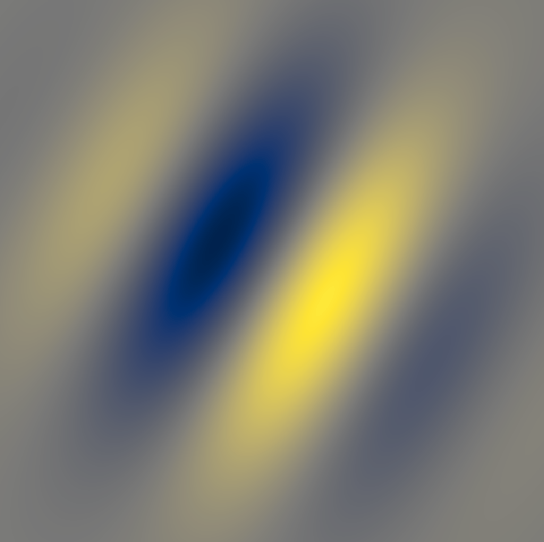
\includegraphics[width=\textwidth]{images/Gabor-2d.png}
                \caption{شکل ۲ بعدی فیلتر گبور}
                \label{fig:part1-Gabor-2d}
            \end{subfigure}
            \hfill % optional; use for aligning images side by side
            \begin{subfigure}[b]{0.5\textwidth}
                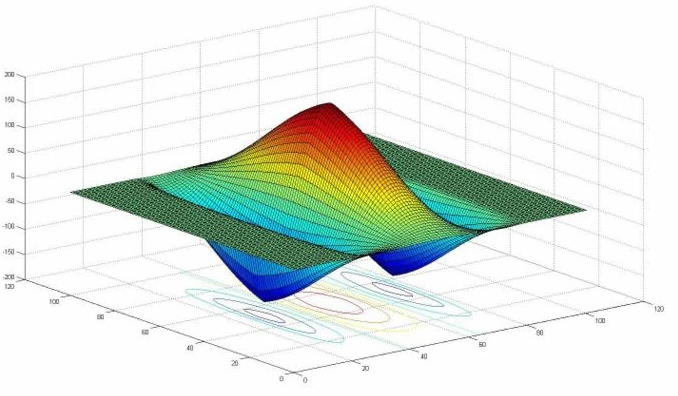
\includegraphics[width=\textwidth]{images/Gabor-3d.jpg}
                \caption{شکل ۳ بعدی فیلتر گبور}
                \label{fig:part1-Gabor-3d}
            \end{subfigure}
            \caption{فیلتر گبور}
            \label{fig:part1-Gabor}
        \end{figure}
        \subsection{دیدگاه ریاضی}
        فیلترهای گبور از نظر ریاضی در توابع پیچیده ای که امواج سینوسی را با پوشش های گاوسی ترکیب می کنند، پایه گذاری می شوند. این ساختار منحصربه‌فرد به آن‌ها اجازه می‌دهد هم فرکانس و هم اطلاعات مکانی را ضبط کنند، و آنها را برای مدل‌سازی پردازش بصری در مغز مناسب می‌سازد. در این بخش، فرمول ریاضی فیلترهای گبور و نحوه استفاده از آنها در وظایف پردازش تصویر را بررسی خواهیم کرد.
        
            \subsubsection*{تابع گبور}
            
            یک فیلتر گبور توسط یک تابع نمایی پیچیده که توسط یک تابع گاوسی مدوله شده است، تعریف می شود. شکل کلی فیلتر گبور دو بعدی را می توان به صورت زیر بیان کرد:
            
            \[ g(x، y؛ \lambda، \theta، \psi، \sigma، \gamma) = \exp \left( -\frac{x'^2 + \gamma^2 y'^2}{2\ sigma^2} \right) \exp \left( i \left( 2\pi \frac{x'}{\lambda} + \psi \right) \right) \]
            
            به طوری که:
            
            \[ x' = x \cos \theta + y \sin \theta \]
            \[ y' = -x \sin \theta + y \cos \theta \]
            
            در این معادله:
            \begin{itemize}
                \item  $\lambda$ (طول موج) فرکانس فضایی موج سینوسی را کنترل می کند.
                    \item  $\theta$  (جهت) جهت فیلتر را نشان می دهد.
                \item  $\psi$ (تغییر فاز) تغییر فاز تابع سینوسی را تعیین می کند.
                \item  $\sigma$ (انحراف معیار) پهنای گاوسی را مشخص می کند.
                \item  $\omega$ (نسبت ابعاد) بیضی بودن تابع گاوسی را تعریف می کند.
            \end{itemize}
            
            \subsubsection*{بخش های حقیقی و موهومی}
            
            یک فیلتر گبور را می توان به بخش های حقیقی و موهومی خود، مطابق با اجزای کسینوس و سینوسی تابع سینوسی، جدا کرد:
            
            \textbf{قسمت حقیقی:}
            \[ g_{\text{real}}(x, y؛ \lambda, \theta, \psi, \sigma, \gamma) = \exp \left( -\frac{x'^2 + \gamma^2 y '^2}{2\sigma^2} \right) \cos \left( 2\pi \frac{x'}{\lambda} + \psi \right) \]
            
            \textbf{قسمت موهومی:}
            \[ g_{\text{imag}}(x, y؛ \lambda, \theta, \psi, \sigma, \gamma) = \exp \left( -\frac{x'^2 + \gamma^2 y '^2}{2\sigma^2} \right) \sin \left( 2\pi \frac{x'}{\lambda} + \psi \right) \]
            
            این اجزا امکان جداسازی پاسخ فیلتر را به فازهای زوج و فرد فراهم می کند و تجزیه و تحلیل جامع تری از ویژگی های تصویر ارائه می دهد.
            
            در نتیجه، فرمول ریاضی فیلترهای گبور شامل ترکیبی از توابع گاوسی و سینوسی است که به آنها امکان می دهد هم اطلاعات مکانی و هم اطلاعات فرکانسی را ضبط کنند. با تنظیم پارامترها، این فیلترها را می توان برای تشخیص جهت گیری ها و مقیاس های مختلف تنظیم کرد و آنها را به ابزاری قدرتمند برای تجزیه و تحلیل تصویر و مدل سازی مکانیسم های پردازش بصری در مغز تبدیل کرد.
        \subsection{تاثیر پارامتر ها}
            حال در این قسمت، تاثیر هر یک از پارامتر ها در فیلتر ها را بررسی می‌کنیم. وابستگی پارامتری این فیلتر و تأثیراتی که این پارامترها بر پاسخ فیلتر دارند را مشخیص می‌کنیم. این پیاده‌سازی با تمرکز بر پارامترهای کلیدی مورد بحث قرار می‌گیرد: اندازه فیلتر، طول موج 
            ($\lambda$)، 
            جهت ($\theta$)، 
            انحراف استاندارد ($\sigma$)، 
            نسبت ابعاد ($\gamma$)، 
            و اندازه گام. هر پارامتر از طریق یک سری آزمایش های کنترل شده طراحی شده برای روشن کردن اثرات فردی آنها بر ویژگی های فیلتر حاصل بررسی می شود.

            نتایج بصری از این آزمایش‌ها برای نشان دادن اثرات ملموس تغییرات پارامترها، ارائه بینش‌هایی در مورد چگونگی تنظیم هر پارامتر برای بهینه‌سازی عملکرد فیلتر برای کاربردهای خاص ارائه شده است.(شکل \ref{fig:part1-Gabor-Kernel})
            \begin{figure}[!ht]
                \centering
                \includegraphics[width=0.9\textwidth]{plots/part1-Gabor-Kernel.pdf} 
                \captionsetup{width=.9\linewidth}
                \caption{\textbf{مقایسه تاثیر پارامتر های فیلتر گبور.} در این شکل، تاثیر هر یک از پارامتر های 
                اندازه فیلتر، طول موج 
                ($\lambda$)، 
                جهت ($\theta$)، 
                انحراف استاندارد ($\sigma$)، 
                نسبت ابعاد ($\gamma$)، 
                بررسی شده است. 
                هر نمودار تغییرات فرکانس مکانی و ویژگی‌های جهت‌گیری فیلتر را نشان می‌دهد و مشخص می‌کند که چگونه مقداردهی پارامتر می‌تواند پاسخ فیلتر را به ویژگی‌های خاص در برنامه‌های پردازش تصویر تنظیم کند. نمایش‌های سه‌بعدی در ردیف پایین، نیز برای درک عمیق تر این تاثیرات آمده است.}
                \label{fig:part1-Gabor-Kernel}
            \end{figure}


        \subsection{خروجی تصویر پس از اعمال فیلتر گبور}
            در این بخش مشابه قسمت قبل یک فیلتر گبور را روی یک تصویر نمونه هم‌گشت(convolve)
            می‌کنیم و خروجی آن را نمایش می‌دهیم.
            برای اینکار، تصویری که در بخش قبل به عنوان نمونه انتخاب کردیم را در اینجا نیز آورده و فیلتر گبور را با دو نسخه 
            off-center و on-center 
            روی آن اعمال می‌کنیم. شکل 
            \ref{fig:part1-Gabor-convolution}
            تصویر ورودی، هسته گبور و تصاویر فیلتر شده حاصل را نشان می دهد.

            مطابق قسمت قبل، شکل بالا سمت چپ، تصویر نمونه را نشان می‌دهد.
            سپس هسته گبور مورد استفاده برای کانولوشن نمایش داده می شود. این کرنل با پارامترهایی مانند طول موج، جهت گیری، فاصله فاز و نسبت ابعاد مشخص می شود که نحوه تعامل فیلتر با تصویر ورودی را مشخص می کند. نمایش بصری هسته گبور جهت گیری و ویژگی های فرکانس آن را برجسته می کند و نمای واضحی از عملکرد فیلتر ارائه می دهد.
            
            سپس شکل خروجی فیلتر گبور 
            on-center
            اعمال شده روی تصویر ورودی را نشان می دهد. در این نسخه، فیلتر ویژگی‌های مرکزی تصویر را افزایش می‌دهد و مناطقی را برجسته می‌کند که با جهت‌گیری و ویژگی‌های فرکانس فیلتر مطابقت دارند. نتیجه فیلتر در مرکز بر قسمت مرکزی میدان گیرنده تأکید می‌کند و آن را به ویژگی‌های بصری خاص همسو با پارامترهای فیلتر حساس می‌کند.

            در ادامه خروجی فیلتر گبور 
            off-center
            ارائه می شود. این نسخه از فیلتر ویژگی‌های مرکزی را سرکوب می‌کند و بر نواحی اطراف تأکید می‌کند. نتیجه فیلتر
            off-center
            نشان می‌دهد که چگونه فیلتر به لبه‌ها و بافت‌های اطراف ناحیه مرکزی پاسخ می‌دهد و جنبه‌های مختلف ویژگی‌های تصویر را به تصویر می‌کشد.

            نتایج به وضوح نشان می‌دهد که چگونه می‌توان از فیلترهای گبور برای استخراج ویژگی‌های خاص از تصاویر، مانند لبه‌ها و بافت‌ها، بسته به پارامترهای انتخابی استفاده کرد. مقادیر مختلف سیگما بر وسعت فضایی و محلی‌سازی فیلتر تأثیر می‌گذارد، در حالی که نسخه‌های 
            on-center
            و 
            off-center
            ، دیدگاه‌های متمایزی را در مورد ویژگی‌های تصویر ارائه می‌کنند. با تغییر مقادیر سیگما و مقایسه خروجی های 
            on-center
            و 
            off-center
            ، می توانیم مشاهده کنیم که چگونه تنظیمات مختلف فیلتر گبور جنبه های مختلف تصویر را برجسته می کند.
            \begin{figure}[!ht]
                \centering
                \includegraphics[width=0.8\textwidth]{plots/part1-Gabor-convolution.pdf} 
                \captionsetup{width=.8\linewidth}
                \caption{\textbf{کاربرد فیلترهای گبور با سیگماهای مختلف و نسخه های On-Center/Off-Center.} 
                شکل، مراحل پردازش و نتایج اعمال فیلترهای گبور بر روی یک تصویر نمونه را نشان می دهد. 
                (ستون اول از سمت چپ) 
                تصویر ورودی اصلی. 
                (ستون دوم از سمت چپ) 
                هسته گبور مورد استفاده برای کانولوشن، که با پارامترهای خاصی برای طول موج، جهت‌گیری، تغییر فاز و نسبت ابعاد مشخص می‌شود. 
                (ستون سوم از سمت چپ) 
                خروجی فیلتر گبور 
                on-center
                که ویژگی‌های مرکزی هماهنگ با ویژگی‌های فیلتر را افزایش می‌دهد. 
                (ستون چهارم از سمت چپ) 
                خروجی فیلتر گبور 
                off-center
                که ویژگی های مرکزی را سرکوب می کند و بر مناطق اطراف تأکید می کند. مقادیر مختلف سیگما استفاده شده در فیلترها بر وسعت فضایی و محلی‌سازی تأثیر می‌گذارد و توانایی فیلترها در برجسته کردن ویژگی‌های مختلف تصویر را نشان می‌دهد.}
                \label{fig:part1-Gabor-convolution}
            \end{figure}

    \clearpage
    \section{خروجی تصاویر فیلتر شده براساس ضربه(spike)}
        در این بخش، نتایج اعمال فیلتر تفاضل گاوسی 
        (DoG) 
        و گبور و کدگذاری ضربه‌ای را با استفاده از روش 
        Time-to-First-Spike
        بر روی یک تصویر نمونه ارائه می‌کنیم. هدف نشان دادن تأثیر فیلتر ها 
        بر افزایش ویژگی‌های بصری و اثربخشی آن در جهت بهبود پاسخ‌های عصبی ساختاریافته‌تر و کارآمدتر است. با مقایسه نمودارهای ضربه های عصبی تولید شده از تصاویر فیلتر نشده و فیلترشده 
        ما پیشرفت‌ها را در 
        % هم ترازی زمانی و
        سازمان‌دهی الگوی ضربه‌ها برجسته می‌کنیم، و به اهمیت پیش پردازش الهام‌گرفته شده از بیولوژیکی پی میبریم.

        شکل 
        \ref{fig:part1-compare-ttfs-filters-spikes}
        کدگذاری عصبی یک تصویر نمونه پردازش شده با و بدون فیلتر تفاضل گاوسی 
        (DoG) 
        را با استفاده از روش
        Time-to-First-Spike
        نشان می‌دهد. 

        نمودار سمت چپ، پاسخ های عصبی به ورودی حسی را بدون اعمال فیلتر پیش پردازش نشان می دهد. در این نمودار، هر نقطه نشان دهنده یک ضربه از یک نورون است که با محور های زمان 
        (محور x )
        و 
        نورون
        (محور y ) 
        ترسیم شده است. توزیع و چگالی ضربه ها پراکنده است، که نشان دهنده یک پاسخ عصبی ساختاری کمتر به ورودی بصری خام است. نورون‌ها در زمان‌های مختلف ضربه می‌زنند و ماهیت پردازش نشده اطلاعات بصری را منعکس می‌کنند که منجر به یک الگوی گسترده و کمتر هماهنگ از فعالیت می‌شود.

        نمودار سمت راست، پاسخ‌های عصبی به همان ورودی حسی را پس از پردازش با فیلتر 
        DoG 
        نشان می‌دهد. این مرحله پیش پردازش لبه ها و کنتراست را در تصویر افزایش می دهد و در نتیجه پاسخ عصبی ساختاریافته تر و کارآمدتری ایجاد می کند. ضربه‌ها از نظر زمانی بیشتر در یک راستا قرار دارند و نشان می‌دهد که نورون‌ها به طور همزمان به ویژگی‌های بهبود یافته تصویر پاسخ می‌دهند. این همگام سازی نشان می دهد که فیلتر 
        DoG 
        به برجسته کردن ویژگی های بصری برجسته کمک می کند و آنها را برای سیستم کدگذاری عصبی بیشتر قابل تشخیص می کند. الگوی کلی ضربه‌ها سازماندهی‌تر است و نمایش عصبی منسجمی از تصویر پردازش‌شده را نشان می‌دهد.

        مقایسه بین دو نمودار تأثیر فیلتر 
        DoG 
        بر کدگذاری عصبی را برجسته می کند. ورودی فیلتر نشده منجر به یک پاسخ عصبی پراکنده و کمتر سازمان‌دهی شده می‌شود، در حالی که ورودی فیلتر شده توسط 
        DoG 
        منجر به الگوی دقیق‌تر و ساختار یافته‌تر می‌شود. این نشان می دهد که فیلتر 
        DoG 
        به طور موثر ویژگی های مهم در ورودی بصری را افزایش می دهد و نمایش عصبی کارآمدتر و دقیق تر را تسهیل می کند. روش 
        time-to-first-spike 
        این پیشرفت‌ها را نشان می‌دهد و نشان می‌دهد که چگونه مراحل پیش‌پردازش مانند فیلتر 
        DoG 
        می‌تواند کدگذاری عصبی اطلاعات بصری را بهبود بخشد.

        \begin{figure}[!ht]
            \centering
            \includegraphics[width=\textwidth]{plots/part1-compare-ttfs-filters-spikes.png} 
            \captionsetup{width=.9\linewidth}
            \caption{\textbf{مقایسه نمودار رستر برای ۳ حالت بدون فیلتر، با فیلتر 
            DoG 
            و با فیلتر گبور.} 
            نمودارهای رستر کدگذاری عصبی یک تصویر نمونه را با استفاده از روش 
            Time-to-First-Spike
            نمایش می دهند. 
            (سمت چپ) 
            پاسخ‌های عصبی بدون فیلتر پیش‌پردازش، الگوی پراکنده و ساختار کمتری از ضربه‌ها را نشان می‌دهد. 
            (وسط و راست) 
            پاسخ‌های عصبی پس از اعمال فیلتر 
            DoG 
            و گبور نشان دادن یک الگوی سازمان‌یافته‌تر و هماهنگ‌تر زمانی از ضربه ها و برجسته کردن ویژگی‌های بهبود یافته تصویر. فیلتر ها
            با تأکید بر لبه ها و کنتراست ها در ورودی بصری، کارایی و دقت کدگذاری عصبی را بهبود می بخشد.}
            \label{fig:part1-compare-ttfs-filters-spikes}
        \end{figure}

        پس از کدگذاری عصبی تصویر نمونه، به سراغ کدگشایی
        (Decoding)
        برای بازسازی اطلاعات بصری از ضربه های کدگذاری شده می‌رویم. هدف این فرآیند نشان دادن پایداری بازنمایی عصبی و اثربخشی فیلتر 
        DoG 
        در حفظ ویژگی‌های بصری حیاتی در طول مراحل کدگذاری و کدگشایی است. شکل
        \ref{fig:part1-compare-ttfs-filters-decoded}
        مجموعه‌ای از تصاویر بازسازی‌شده از ضربه ها را در تکرارهای مختلف نشان می‌دهد.

        \begin{figure}[!ht]
            \centering
            \begin{subfigure}[b]{\textwidth}
                \includegraphics[width=\textwidth]{plots/part1-compare-ttfs-dog-decoded.pdf}
                \caption{استفاده از فیلتر DoG}
                \label{fig:part1-compare-ttfs-dog-decoded}
            \end{subfigure}
            \vfill % optional; use for aligning images side by side
            \begin{subfigure}[b]{\textwidth}
                \includegraphics[width=\textwidth]{plots/part1-compare-ttfs-gabor-decoded.pdf}
                \caption{استفاده از فیلتر گبور}
                \label{fig:part1-compare-ttfs-gabor-decoded}
            \end{subfigure}
            \caption{\textbf{تصاویر بازسازی شده از ضربه های ورودی فیلتر شده با استفاده از دیکودر 
            TTFS} 
            شکل، کدگشایی ضربه های عصبی کدگذاری شده با استفاده از روش 
            Time-to-First-Spike 
            را نشان می دهد. 
            (تصویر اول از سمت چپ) 
            تصویر ورودی اصلی. 
            (تصویر دوم از سمت چپ) 
            فیلتر مورد استفاده.
            (تصویر سوم از سمت چپ)
            تصویر با فیلتر 
            DoG یا گبور
            هم‌گشت شده
            (convolve)
            و لبه ها و کنتراست ها را افزایش می دهد. 
            (تصویر چهارم از سمت چپ) 
            تصویر بازسازی شده از ضربه ها توسط دیکودر.
            (ردیف دوم)
            بازسازی تصاویز از ضربه های عصبی با استفاده از دیکودر. در هر تکرار، تصویری که کد شده است بازسازی شده.}
            \label{fig:part1-compare-ttfs-filters-decoded}
        \end{figure}


    \clearpage
    \section{امتیازی}
        \subsection{خروجی ﺗﺼﺎﻭﯾﺮ ﻓﯿﻠﺘﺮ ﺷﺪﻩ ﺑﺮﺍﺳﺎﺱ ﺿﺮبه: انکودر پواسون}
        در این بخش، تجزیه و تحلیل خود را از کدگذاری و کدگشایی عصبی با اعمال یک انکودر
        (Encoder)
        پواسون
        \footnote{Poisson}
        در همان تصویر نمونه ادامه می‌دهیم. انکودر پواسون روشی است که به برای شبیه سازی ضربه های عصبی بر اساس سرعت ضربه زدن نورون ها استفاده می شود. بر خلاف روش زمان تا اولین ضربه 
        (TTFS) 
        که اطلاعات را بر اساس زمان‌بندی اولین ضربه کدگذاری می‌شدند انکودر پواسون طبق یک مدل احتمالی که در آن نرخ ضربه زدن با شدت محرک بینایی مطابقت دارد، ضربه ها را تولید می‌کند. با مقایسه نتایج از انکودر پواسون با نتایج به‌دست‌آمده با استفاده از روش 
        TTFS، 
        هدف ما بررسی روش های مختلف کدگذاری در حفظ اطلاعات بصری از طریق پردازش عصبی است.

        شکل
        \ref{fig:part1-compare-poisson-filters-spikes}
        ضربه های کدگذاری شده یک تصویر نمونه را با استفاده از انکودر پواسون نشان می دهد و اثرات بدون فیلتر، فیلتر تفاوت گاوسی ها 
        (DoG)
        و فیلتر گبور را با هم مقایسه می کند. هر نمودار رستر نشان دهنده ضربه های تولید شده توسط انکودر پواسون تحت شرایط فیلتر های مختلف است.

        اولین نمودار رستر، ضربه های تولید شده از تصویر خام را بدون فیلتر پیش پردازش نشان می دهد. نمودار دوم پس از پردازش تصویر با فیلتر DoG، 
        ضربه ها را نشان می دهد و لبه ها و کنتراست ها را برجسته می کند. نمودار سوم، فعالیت نورون ها پس از اعمال فیلتر گبور را نشان می‌دهد که بر فرکانس‌ها و جهت‌گیری‌های فضایی خاص در تصویر تمرکز می‌کند. این مقایسه‌ها نشان می‌دهد که چگونه فیلترهای مختلف بر فعالیت نورون ها و کدگذاری عصبی حاصل از اطلاعات بصری تأثیر می‌گذارند.

        \begin{figure}[!ht]
            \centering
            \includegraphics[width=\textwidth]{plots/part1-compare-poisson-filters-spikes.png} 
            \captionsetup{width=.9\linewidth}
            \caption{\textbf{مقایسه نمودار رستر برای ۳ حالت بدون فیلتر، با فیلتر 
            DoG 
            و با فیلتر گبور و انکودر پواسون.} 
            نمودارهای رستر، ضربه های تولید شده توسط انکودر پواسون برای یک تصویر نمونه را در سه شرایط نشان می دهند: 
            (سمت چپ) 
            فیلتری اعمال نشده است، که پاسخ عصبی خام را نشان می دهد. 
            (وسط و راست) 
            فیلتر 
            DoG 
            اعمال شده، لبه ها و کنتراست ها را در تصویر افزایش می دهد.
            همانند شکل 
            \ref{fig:part1-compare-ttfs-filters-spikes} 
            در اینجا نیز پس از اعمال فیلتر ها، یک الگوی ساختار یافته تر از ضربه ها مشاهده می‌کنیم. فیلتر ها
            با تأکید بر لبه ها و کنتراست ها در ورودی بصری، کارایی و دقت کدگذاری عصبی را بهبود می بخشد.
            }
            \label{fig:part1-compare-poisson-filters-spikes}
        \end{figure}

        حال مشابه قبل، به دیکود کردن ضربه های حاصل از تصاویر فیلتر شده می‌پردازیم. شکل
        \ref{fig:part1-compare-poisson-filters-decoded}
        نتایج کدگشایی ضربه های عصبی را نشان می دهد که با استفاده از دیکودر پواسون، پس از اعمال فیلتر 
        DoG 
        و گبور بر روی تصویر ورودی، کدگذاری شده اند. کدگشایی با استفاده از دیکودر پواسون انجام می شود، که اطلاعات بصری را از ضربه های تولید شده به صورت احتمالی بازسازی می کند. شکل تصویر اصلی، تصویر فیلتر شده توسط فیلتر ها و تصویر دیکود شده و بازسازی تصویر از ضربه ها در تکرارهای مختلف نشان می دهد. مشابه انکودر
        TTFS
        در اینجا نیز تصویر اصلی از فعالیت نورون ها بازسازی می‌شود. هر چند نسبت به حالت قبل شاهد شباهت کمتری به تصویر ورودی داده شده هستیم که بدلیل ماهیت کدگذاری پواسون می‌باشد.


        \begin{figure}[!ht]
            \centering
            \begin{subfigure}[b]{\textwidth}
                \includegraphics[width=\textwidth]{plots/part1-compare-poisson-dog-decoded.pdf}
                \caption{استفاده از فیلتر DoG}
                \label{fig:part1-compare-poisson-dog-decoded}
            \end{subfigure}
            \vfill % optional; use for aligning images side by side
            \begin{subfigure}[b]{\textwidth}
                \includegraphics[width=\textwidth]{plots/part1-compare-poisson-gabor-decoded.pdf}
                \caption{استفاده از فیلتر گبور}
                \label{fig:part1-compare-poisson-gabor-decoded}
            \end{subfigure}
            \caption{\textbf{تصاویر بازسازی شده از ضربه های ورودی فیلتر شده با استفاده از دیکودر پواسون.} 
            شکل، کدگشایی ضربه های عصبی کدگذاری شده با استفاده از روش پواسون
            را نشان می دهد. 
            (تصویر اول از سمت چپ) 
            تصویر ورودی اصلی. 
            (تصویر دوم از سمت چپ) 
            فیلتر مورد استفاده.
            (تصویر سوم از سمت چپ)
            تصویر با فیلتر 
            DoG یا گبور
            هم‌گشت شده
            (convolve)
            و لبه ها و کنتراست ها را افزایش می دهد. 
            (تصویر چهارم از سمت چپ) 
            تصویر بازسازی شده از ضربه ها توسط دیکودر.
            (ردیف دوم)
            بازسازی تصاویز از ضربه های عصبی با استفاده از دیکودر. در هر تکرار، تصویری که کد شده است بازسازی شده.}
            \label{fig:part1-compare-poisson-filters-decoded}
        \end{figure}

        \subsection{فیلتر های DoG رنگی}
            در این بخش، با الهام از معماری عملکردی سلول های گانگلیونی، به ویژه مسیرهای 
            M\footnote{\lr{magnocellular}}
            و 
            P\footnote{\lr{parvocellular}}، 
            فیلترهای 
            DoG
            را در شبکه عصبی
            خود پیاده سازی کردیم. این رویکرد، ویژگی‌های میدان پذیرای مرکز احاطه سلول‌های گانگلیونی را مدل‌سازی می‌کند، که برای تقویت کنتراست و گرفتن الگوهای فضایی در محرک‌های بصری بسیار مهم هستند.
            \subsubsection*{فیلتر های DoG رنگی}
                همانطور که در بخش قبل نیز توضیح دادیم، فیلتر تفاضل گاوسی مدلی است که پاسخ عصبی سلول های گانگلیونی در شبکیه را تقریب می زند. این مدل شامل تفریق یک نسخه تار از یک تصویر از یک نسخه دیگر با تاری کمتر از همان تصویر است، در نتیجه مناطقی از کنتراست فضایی را برجسته می‌کند که مربوط به میدان‌های گیرنده سلول‌های گانگلیونی است.
                \paragraph*{سلول های M :} این سلول ها به تغییرات شدت نور حساس هستند و با استفاده از فیلترهای استاندارد DoG 
                مقیاس خاکستری مدل سازی می شوند. میدان های گیرنده سلول های 
                M 
                را می توان به دو نوع طبقه بندی کرد:
                \begin{itemize}
                    \item \textbf{سلول‌های \lr{on-center}:} وقتی در معرض نور قرار می‌گیرند، دارای یک مرکز پاسخ‌دهنده مثبت و یک محیط اطراف با پاسخ منفی هستند که از پاسخ جلوگیری می‌کند و تشخیص اجسام روشن در پس‌زمینه‌های تاریک را افزایش می‌دهد.
                    \item \textbf{سلول‌های \lr{off-center}:} دارای یک مرکز پاسخ منفی و یک محیط اطراف با پاسخ مثبت هستند که تشخیص اجسام تاریک را در پس زمینه های روشن افزایش می دهد.
                \end{itemize}
                \paragraph*{سلول های P}
                    این سلول ها نه تنها به شدت نور، بلکه به تضاد رنگ نیز حساس هستند. آنها با استفاده از فیلترهای 
                    RGB DoG 
                    نشان داده می شوند که مخالفت رنگی آنها را منعکس می کند:
                    \begin{itemize}
                        \item \textbf{سلول‌های \lr{on-center}:}  این سلول‌ها شامل سلول‌هایی می‌شوند که به یک رنگ در مرکز پاسخ مثبت و به رنگ دیگری در اطراف پاسخ منفی می‌دهند 
                        (به عنوان مثال، 
                        R+G- 
                        برای قرمز در مرکز، سبز خارج از مرکز).
                        \item \textbf{سلول‌های \lr{off-center}:} این سلول‌ها پاسخی مخالف دارند، با مرکز منفی و اطراف مثبت برای رنگ‌های مکمل 
                        (مانند G+R-).
                    \end{itemize}
                \begin{figure}[!ht]
                    \centering
                    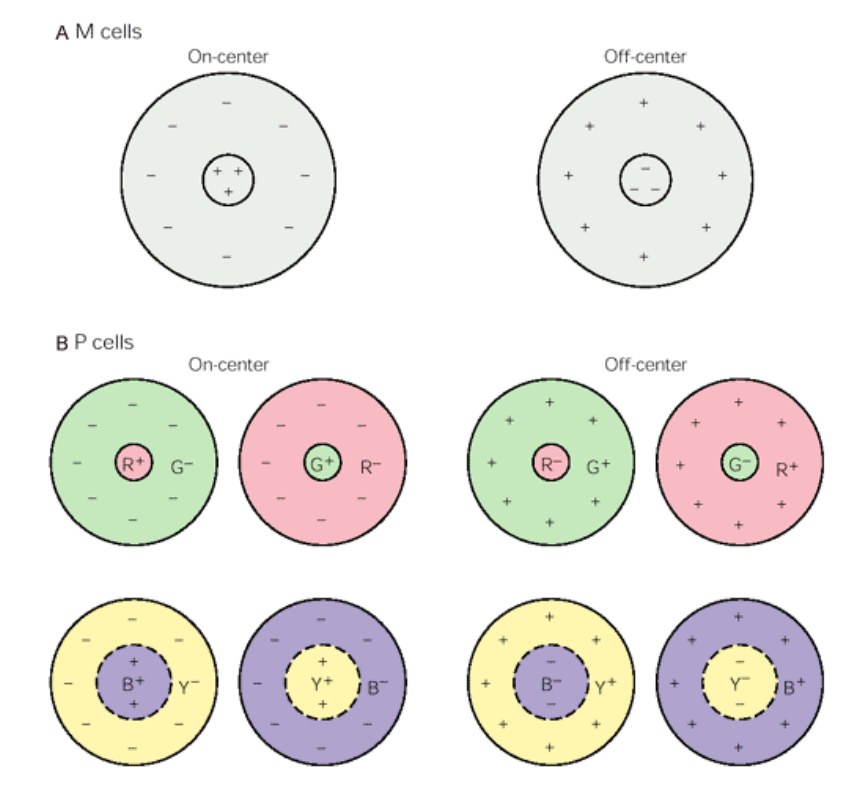
\includegraphics[width=0.5\textwidth]{images/DoG-RGB.png} 
                    \captionsetup{width=.8\linewidth}
                    \caption{\textbf{میدان گیرنده سلول های گانگلیونی.} 
                    این نمودار میدان های پذیرنده سلول های گانگلیونی 
                    M و P 
                    را نشان می دهد. عکس 
                    A 
                    سلول های 
                    M 
                    را با پیکربندی استاندارد روی مرکز و خارج از مرکز حساس به شدت نور نشان می دهد. عکس 
                    B 
                    سلول‌های 
                    P 
                    را با میدان‌های دریافتی مخالف رنگ برای تضادهای قرمز-سبز و آبی-زرد به تصویر می‌کشد که پاسخ‌های مرکز و خارج از مرکز آنها را به محرک‌های رنگی منعکس می‌کند.
                    }
                    \label{fig:part1-DoG-RGB}
                \end{figure}
                در  این قسمت ما از عملیات کانوولوشن با استفاده از فیلتر 
                DoG 
                بر روی یک تصویر به منظور بررسی تاثیر آن در برجسته سازی و بهبود ویژگی‌های بصری خاص که قابلیت‌های پردازشی سلول‌های گانگلیون 
                P 
                در شبکیه انسان را شبیه سازی می‌کند، استفاده کردیم.
                (شکل \ref{fig:part1-DoG-RGB-convolution})
                این فیلتر 
                DoG 
                رنگی، که برای تشخیص تضادهای رنگی و جزئیات مکانی طراحی شده است، به طور جداگانه بر روی کانال‌های قرمز و سبز تصویر اعمال شد. فرایند شامل تقویت نواحی که رنگ‌های مشخص در آنها غالب بود و سرکوب سایر نواحی می‌شد، که این امر تضاد کروماتیک مشاهده شده در سلول‌های 
                P 
                را تکرار می‌کند. نتایج این کانوولوشن نشان می‌دهد که چگونه برخی رنگ‌ها بیشتر برجسته می‌شوند، در حالی که برخی دیگر عقب‌تر می‌روند، و به طور مؤثر نشان می‌دهد که چگونه پردازش مشابه گانگلیون می‌تواند در سیستم‌های بصری مصنوعی برای اولویت‌بندی و تفکیک اطلاعات بصری بر اساس پویایی رنگ‌ها استفاده شود.

                \begin{figure}[!ht]
                    \centering
                    \includegraphics[width=0.6\textwidth]{plots/part1-DoG-RGB.pdf} 
                    \captionsetup{width=.7\linewidth}
                    \caption{\textbf{کاربرد کانولوشن فیلتر 
                    DoG
                    رنگی روی یک تصویر.} 
                    عکس سمت چپ تصویر اصلی را نشان می دهد، در حالی که عکس  سمت راست یا پایین نتایج را پس از اعمال فیلتر رنگی تفاوت گاوسی 
                    (DoG) 
                    روی کانال های قرمز و سبز نشان می دهند. همانطور که از شکل نیز پیداست، فیلتر توانسته است به خوبی بین روی تصویر اعمال شود. این نشان دهنده ظرفیت فیلتر برای افزایش و متمایز کردن ویژگی های خاص رنگ، تقلید از مخالفت رنگی سلول های گانگلیونی 
                    P 
                    در لایه های اولیه بینایی است.
                    }
                    \label{fig:part1-DoG-RGB-convolution}
                \end{figure}